% 箇条書き
\begin{itemize}
\item Item.
\item Another Item.
\end{itemize}

%番号付きリスト
\begin{enumerate}
\item First Item
\item Second Item
\end{enumerate}

% Section,subsection,paragraph
\section{Section Title}
One Section
\paragraph{paragraph title}
nekomajin
\paragraph{paragraph title}
nekomajinn

\subsection{subsec title}
Subsec one
\paragraph{pragraph title}
nekomajin 
nekonyan 
neko
\subparagraph{subpragraph title}
nekoneko
\subparagraph{subpragraph title}
nekoneko
\paragraph{paragraph title}
nekomajin neko nyan

% 改ページ
\newpage

% 脚注、改行
Hi let me introduce myself
\footnote{\label{myfootnote}Hello footnote}.
\newline
... (later on)\\
I'm referring to myself\ref{myfootnote}.
\newline
\newline

% 数式
\begin{align*}
x&=y & w&=z & a&=b+c\\
2x&=-y & 3w&=\frac{1}{2}z & a&=b\\
-4 + 5x&=2+y & w+2&=-1+w & ab&=cb
\end{align*}

\begin{equation}
\begin{split}
A & = \frac{\pi r^2}{2}\\
 & = \frac{1}{2} \pi r^2
 \end{split}
\end{equation}

% テーブル
\begin{table}[t!]%h,t,b,p
  \centering
  \caption{Caption for the table.}
  \label{tab:table1}
  \begin{tabular}{l|c||r||c}
    1 & 2 & 3\\
    \hline
    a & b & c\\
    \hline
    neko nyan neko& neko & nyan & nekon\\
  \end{tabular}
\end{table}

% 画像追加
\begin{figure}[t!]
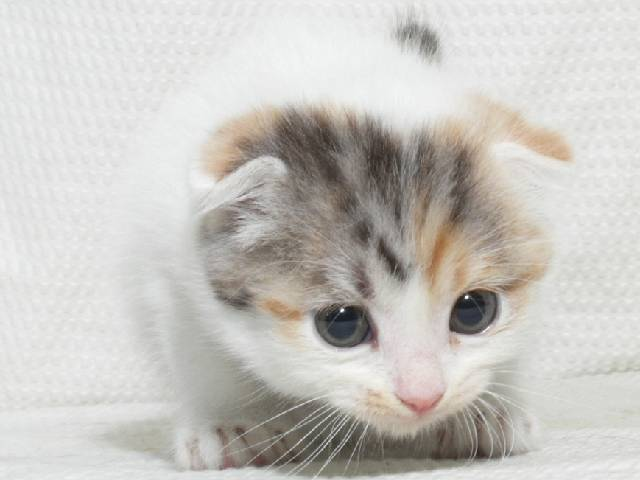
\includegraphics[width=\linewidth]{neko.jpg}
\caption{What is it about?}
\label{fig:whateverlabel}
\end{figure}

% 開発ソースの挿入
\begin{verbatim}
#include <iostream>
 
int main()
{
    std::cout << "hello world! \n";
    return 0;
}
\end{verbatim}

